\PassOptionsToPackage{unicode=true}{hyperref} % options for packages loaded elsewhere
\PassOptionsToPackage{hyphens}{url}
\PassOptionsToPackage{dvipsnames,svgnames*,x11names*}{xcolor}
%
\documentclass[10pt,ignorenonframetext,]{beamer}
\usepackage{pgfpages}
\setbeamertemplate{caption}[numbered]
\setbeamertemplate{caption label separator}{: }
\setbeamercolor{caption name}{fg=normal text.fg}
\beamertemplatenavigationsymbolsempty
% Prevent slide breaks in the middle of a paragraph:
\widowpenalties 1 10000
\raggedbottom
\setbeamertemplate{part page}{
\centering
\begin{beamercolorbox}[sep=16pt,center]{part title}
  \usebeamerfont{part title}\insertpart\par
\end{beamercolorbox}
}
\setbeamertemplate{section page}{
\centering
\begin{beamercolorbox}[sep=12pt,center]{part title}
  \usebeamerfont{section title}\insertsection\par
\end{beamercolorbox}
}
\setbeamertemplate{subsection page}{
\centering
\begin{beamercolorbox}[sep=8pt,center]{part title}
  \usebeamerfont{subsection title}\insertsubsection\par
\end{beamercolorbox}
}
\AtBeginPart{
  \frame{\partpage}
}
\AtBeginSection{
  \ifbibliography
  \else
    \frame{\sectionpage}
  \fi
}
\AtBeginSubsection{
  \frame{\subsectionpage}
}
\usepackage{lmodern}
\usepackage{amssymb,amsmath}
\usepackage{ifxetex,ifluatex}
\usepackage{fixltx2e} % provides \textsubscript
\ifnum 0\ifxetex 1\fi\ifluatex 1\fi=0 % if pdftex
  \usepackage[T1]{fontenc}
  \usepackage[utf8]{inputenc}
  \usepackage{textcomp} % provides euro and other symbols
\else % if luatex or xelatex
  \usepackage{unicode-math}
  \defaultfontfeatures{Ligatures=TeX,Scale=MatchLowercase}
\fi
\usetheme[]{Singapore}
\usefonttheme{serif}
% use upquote if available, for straight quotes in verbatim environments
\IfFileExists{upquote.sty}{\usepackage{upquote}}{}
% use microtype if available
\IfFileExists{microtype.sty}{%
\usepackage[]{microtype}
\UseMicrotypeSet[protrusion]{basicmath} % disable protrusion for tt fonts
}{}
\IfFileExists{parskip.sty}{%
\usepackage{parskip}
}{% else
\setlength{\parindent}{0pt}
\setlength{\parskip}{6pt plus 2pt minus 1pt}
}
\usepackage{xcolor}
\usepackage{hyperref}
\hypersetup{
            pdftitle={Module 12: Summing up and some cautionary notes},
            pdfauthor={Stefanie Muff, Department of Mathematical Sciences, NTNU},
            colorlinks=true,
            linkcolor=Maroon,
            filecolor=Maroon,
            citecolor=Blue,
            urlcolor=blue,
            breaklinks=true}
\urlstyle{same}  % don't use monospace font for urls
\newif\ifbibliography
\usepackage{color}
\usepackage{fancyvrb}
\newcommand{\VerbBar}{|}
\newcommand{\VERB}{\Verb[commandchars=\\\{\}]}
\DefineVerbatimEnvironment{Highlighting}{Verbatim}{commandchars=\\\{\}}
% Add ',fontsize=\small' for more characters per line
\usepackage{framed}
\definecolor{shadecolor}{RGB}{248,248,248}
\newenvironment{Shaded}{\begin{snugshade}}{\end{snugshade}}
\newcommand{\AlertTok}[1]{\textcolor[rgb]{0.94,0.16,0.16}{#1}}
\newcommand{\AnnotationTok}[1]{\textcolor[rgb]{0.56,0.35,0.01}{\textbf{\textit{#1}}}}
\newcommand{\AttributeTok}[1]{\textcolor[rgb]{0.77,0.63,0.00}{#1}}
\newcommand{\BaseNTok}[1]{\textcolor[rgb]{0.00,0.00,0.81}{#1}}
\newcommand{\BuiltInTok}[1]{#1}
\newcommand{\CharTok}[1]{\textcolor[rgb]{0.31,0.60,0.02}{#1}}
\newcommand{\CommentTok}[1]{\textcolor[rgb]{0.56,0.35,0.01}{\textit{#1}}}
\newcommand{\CommentVarTok}[1]{\textcolor[rgb]{0.56,0.35,0.01}{\textbf{\textit{#1}}}}
\newcommand{\ConstantTok}[1]{\textcolor[rgb]{0.00,0.00,0.00}{#1}}
\newcommand{\ControlFlowTok}[1]{\textcolor[rgb]{0.13,0.29,0.53}{\textbf{#1}}}
\newcommand{\DataTypeTok}[1]{\textcolor[rgb]{0.13,0.29,0.53}{#1}}
\newcommand{\DecValTok}[1]{\textcolor[rgb]{0.00,0.00,0.81}{#1}}
\newcommand{\DocumentationTok}[1]{\textcolor[rgb]{0.56,0.35,0.01}{\textbf{\textit{#1}}}}
\newcommand{\ErrorTok}[1]{\textcolor[rgb]{0.64,0.00,0.00}{\textbf{#1}}}
\newcommand{\ExtensionTok}[1]{#1}
\newcommand{\FloatTok}[1]{\textcolor[rgb]{0.00,0.00,0.81}{#1}}
\newcommand{\FunctionTok}[1]{\textcolor[rgb]{0.00,0.00,0.00}{#1}}
\newcommand{\ImportTok}[1]{#1}
\newcommand{\InformationTok}[1]{\textcolor[rgb]{0.56,0.35,0.01}{\textbf{\textit{#1}}}}
\newcommand{\KeywordTok}[1]{\textcolor[rgb]{0.13,0.29,0.53}{\textbf{#1}}}
\newcommand{\NormalTok}[1]{#1}
\newcommand{\OperatorTok}[1]{\textcolor[rgb]{0.81,0.36,0.00}{\textbf{#1}}}
\newcommand{\OtherTok}[1]{\textcolor[rgb]{0.56,0.35,0.01}{#1}}
\newcommand{\PreprocessorTok}[1]{\textcolor[rgb]{0.56,0.35,0.01}{\textit{#1}}}
\newcommand{\RegionMarkerTok}[1]{#1}
\newcommand{\SpecialCharTok}[1]{\textcolor[rgb]{0.00,0.00,0.00}{#1}}
\newcommand{\SpecialStringTok}[1]{\textcolor[rgb]{0.31,0.60,0.02}{#1}}
\newcommand{\StringTok}[1]{\textcolor[rgb]{0.31,0.60,0.02}{#1}}
\newcommand{\VariableTok}[1]{\textcolor[rgb]{0.00,0.00,0.00}{#1}}
\newcommand{\VerbatimStringTok}[1]{\textcolor[rgb]{0.31,0.60,0.02}{#1}}
\newcommand{\WarningTok}[1]{\textcolor[rgb]{0.56,0.35,0.01}{\textbf{\textit{#1}}}}
\usepackage{graphicx,grffile}
\makeatletter
\def\maxwidth{\ifdim\Gin@nat@width>\linewidth\linewidth\else\Gin@nat@width\fi}
\def\maxheight{\ifdim\Gin@nat@height>\textheight\textheight\else\Gin@nat@height\fi}
\makeatother
% Scale images if necessary, so that they will not overflow the page
% margins by default, and it is still possible to overwrite the defaults
% using explicit options in \includegraphics[width, height, ...]{}
\setkeys{Gin}{width=\maxwidth,height=\maxheight,keepaspectratio}
\setlength{\emergencystretch}{3em}  % prevent overfull lines
\providecommand{\tightlist}{%
  \setlength{\itemsep}{0pt}\setlength{\parskip}{0pt}}
\setcounter{secnumdepth}{0}

% set default figure placement to htbp
\makeatletter
\def\fps@figure{htbp}
\makeatother

\usepackage{multirow}

\title{Module 12: Summing up and some cautionary notes}
\providecommand{\subtitle}[1]{}
\subtitle{TMA4268 Statistical Learning V2022}
\author{Stefanie Muff, Department of Mathematical Sciences, NTNU}
\date{April 21, 2022}

\begin{document}
\frame{\titlepage}

\begin{frame}{Overview}
\protect\hypertarget{overview}{}

\(~\)

\begin{itemize}
\item
  Course content and learning outcome \vspace{2mm}
\item
  Overview of modules and core course topics \vspace{2mm}
\item
  Some cautionary notes
\end{itemize}

\end{frame}

\begin{frame}

Some of the figures and slides in this presentation are taken (or are
inspired) from G. James et al. (2013).

\end{frame}

\begin{frame}{Learning outcomes of TMA4268}
\protect\hypertarget{learning-outcomes-of-tma4268}{}

\begin{enumerate}
\item
  \textbf{Knowledge.} The student has knowledge about the most popular
  statistical learning models and methods that are used for
  \emph{prediction} and \emph{inference} in science and technology.
  Emphasis is on regression- and classification-type statistical models.
\item
  \textbf{Skills.} The student can, based on an existing data set,
  \emph{choose a suitable statistical model, apply sound statistical
  methods}, and \emph{perform the analyses using statistical software}.
  The student can present, interpret and communicate the results from
  the statistical analyses, and knows which conclusions can be drawn
  from the analyses, and what are the caveats.
\end{enumerate}

\(~\)

\textbf{And}: you got to be an expert in using the R language and
writing R Markdown reports.

\end{frame}

\begin{frame}{The exam}
\protect\hypertarget{the-exam}{}

\(~\)

\begin{itemize}
\tightlist
\item
  \textbf{Digital home exam} June 3rd, 9-13h, +30' to scan and upload
  files.
\end{itemize}

\(~\)

Tentative plan:

\begin{itemize}
\tightlist
\item
  Warm up section
\item
  1-2 examples with real data
\item
  A conceptual/theoretical section testing your understanding.
\item
  A section with single/multiple choice questions.
\end{itemize}

\(~\)

Check out the exam from last year (see course website).

\end{frame}

\begin{frame}{The course book}
\protect\hypertarget{the-course-book}{}

\(~\)

Attention:

\begin{itemize}
\item
  We are mainly working with the \emph{first edition}:
  \url{https://www.statlearning.com/}
\item
  The \emph{second edition} came out very recently. Chapter 10 is
  relevant for our Module 11 (Neural networks and deep learning):
\end{itemize}

\centering

\includegraphics[width=0.5\textwidth,height=\textheight]{deep_learning.png}

\end{frame}

\begin{frame}{Core of the course}
\protect\hypertarget{core-of-the-course}{}

Supervised and unsupervised learning:

\begin{itemize}
\tightlist
\item
  \emph{\textcolor{red}{Supervised}}: regression and classification

  \begin{itemize}
  \tightlist
  \item
    examples of regression and classification type problems
  \item
    how complex a model to get the best fit?\\
    \(\rightarrow\) flexiblity/overfitting/underfitting.
  \item
    the bias-variance trade-off
  \item
    how to find a good fit - validation and cross-validation (or
    AIC-type solutions)
  \item
    how to compare different solutions
  \item
    how to evaluate the fit - on new unseen data
  \end{itemize}
\end{itemize}

\vspace{2mm}

\begin{itemize}
\tightlist
\item
  \emph{\textcolor{red}{Unsupervised}}: how to find structure or
  groupings in data?
\end{itemize}

\vspace{2mm}

and of course all \textbf{the methods} (with underlying models) to
perform regression, classification and unsupervised learning.

\end{frame}

\begin{frame}

\centering

\includegraphics{../../ISLR/Figures/Chapter2/2.7.png} Figure 2.7 from
Gareth James et al. (2013)

\end{frame}

\begin{frame}{The modules}
\protect\hypertarget{the-modules}{}

\begin{block}{1. Introduction}

\(~\)

\begin{itemize}
\tightlist
\item
  Examples, the modules, required background in statistics \vspace{2mm}
\item
  Introduction to R and RStudio via the online R-course
\end{itemize}

\end{block}

\end{frame}

\begin{frame}

\begin{block}{2. Statistical learning}

\(~\)

\begin{itemize}
\tightlist
\item
  Model complexity

  \begin{itemize}
  \tightlist
  \item
    Prediction vs.~interpretation (inference).\\
  \item
    Parametric vs.~nonparametric.
  \item
    Flexible vs.~inflexible.
  \item
    Overfitting vs.~underfitting \vspace{2mm}
  \end{itemize}
\item
  Supervised vs.~unsupervised. \vspace{2mm}
\item
  Regression and classification. \vspace{2mm}
\item
  Loss functions: quadratic and 0/1 loss. \vspace{2mm}
\item
  Bias-variance trade-off (polynomial example): mean squared error,
  training and test set. \vspace{2mm}
\item
  Vectors and matrices, rules for mean and covariances, the multivariate
  normal distribution.
\end{itemize}

\end{block}

\end{frame}

\begin{frame}

\begin{block}{3. Linear regression}

\(~\)

\begin{itemize}
\item
  The classical normal linear regression model on vector/matrix form.
  \vspace{2mm}
\item
  Parameter estimators and distribution thereof. Model fit. \vspace{2mm}
\item
  Confidence intervals, hypothesis tests, and interpreting R-output from
  regression. \vspace{2mm}
\item
  Qualitative covariates, interactions. \vspace{2mm}
\item
  This module is a stepping stone for all subsequent uses of regression
  in Modules 6, 7, 8, and 11.
\end{itemize}

\end{block}

\end{frame}

\begin{frame}

\begin{block}{4. Classification (Mainly two-class problems)}

\(~\)

\begin{itemize}
\tightlist
\item
  Bayes classifier: classify to the most probable class to minimize the
  expected 0/1 loss. We usually do not know the probability of each
  class for each input. The Bayes optimal boundary is the boundary for
  the Bayes classifier and the error rate (on a test set) for the Bayes
  classifier is the Bayes error rate.
\end{itemize}

\(~\)

\begin{itemize}
\tightlist
\item
  Two paradigms (not in textbook):

  \begin{itemize}
  \tightlist
  \item
    \emph{\textcolor{red}{Diagnostic}} (directly estimating the
    posterior distribution for the classes). Example: KNN classifier,
    logistic regression.
  \item
    \emph{\textcolor{red}{Sampling}} (estimating class prior
    probabilities and class conditional distribution and then putting
    together with Bayes rule). Examples: LDA, QDA with linear or
    quadratic class boundaries.
  \end{itemize}
\end{itemize}

\(~\)

\begin{itemize}
\tightlist
\item
  ROC curves, AUC, sensitivity and specificity of classification
  methods.
\end{itemize}

\end{block}

\end{frame}

\begin{frame}

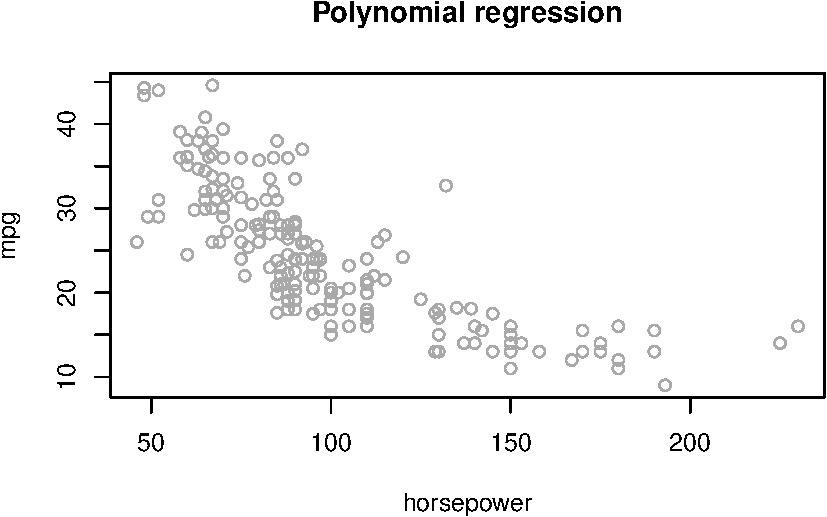
\includegraphics{12Final_files/figure-beamer/unnamed-chunk-1-1.pdf}

\end{frame}

\begin{frame}

Logistic regression gives a probability, given a certain value of the
covariats \(P(Y=1 \, | \, \boldsymbol{x})\).

\includegraphics[width=0.9\textwidth,height=\textheight]{beetles.png}

\end{frame}

\begin{frame}

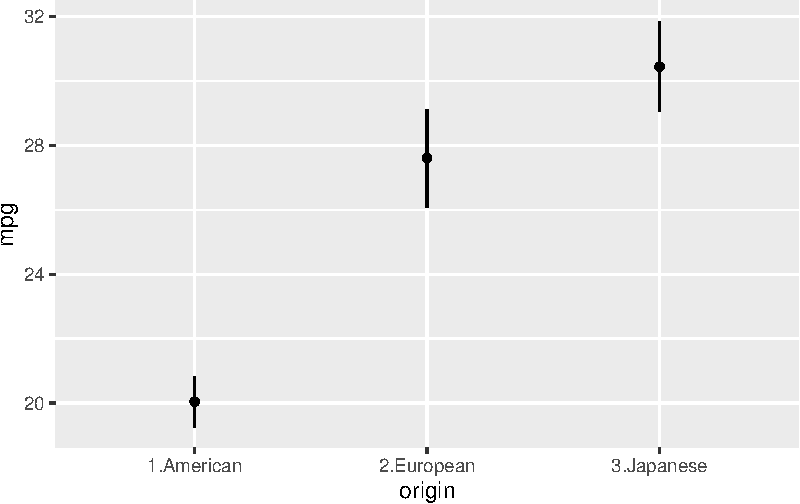
\includegraphics{12Final_files/figure-beamer/unnamed-chunk-3-1.pdf}

\end{frame}

\begin{frame}

\begin{block}{5. Resampling methods}

\(~\)

\textbf{Cros-validation}

\vspace{2mm}

\begin{itemize}
\item
  Data rich situation: Training, validation and test set. \vspace{2mm}
\item
  Validation set approach. \vspace{2mm}
\item
  Cross-validation for regression and for classification. \vspace{2mm}
\item
  LOOCV, 5 and 10 fold CV. \vspace{2mm}
\item
  Good and bad issues with validation set, LOOCV, 10-fold CV.
  \vspace{2mm}
\item
  Bias and variance for \(k\)-fold cross-validation. \vspace{2mm}
\item
  Selection bias -- the right and wrong way to do cross-validation.
  \vspace{2mm}
\item
  Distinction between model selection and model assessment.
\end{itemize}

\(~\)

\textbf{The Bootstrap}

\begin{itemize}
\tightlist
\item
  Idea: Re-use the same data to estimate a statistic of interest by
  \emph{sampling with replacement}.
\end{itemize}

\end{block}

\end{frame}

\begin{frame}

\begin{block}{6. Linear model selection and regularization:}

\(~\)

Subset-selection. Discriminate: \vspace{2mm}

\begin{itemize}
\tightlist
\item
  \emph{\textcolor{red}{Model selection}}: estimate performance of
  different models to choose the best one.
\item
  \emph{\textcolor{red}{Model assessment}}: having chosen a final model,
  estimate its performance on new data.
\end{itemize}

\(~\)

How?

\vspace{2mm}

\begin{itemize}
\tightlist
\item
  Model selection by

  \begin{itemize}
  \tightlist
  \item
    Subset selection (best subset selection or stepwise model selection)
  \item
    Penalizing the training error: AIC, BIC, \(C_p\), Adjusted \(R^2\).
  \item
    Cross-validation.
  \end{itemize}
\end{itemize}

\vspace{2mm}

\begin{itemize}
\tightlist
\item
  Model assessment by

  \begin{itemize}
  \tightlist
  \item
    Cross-validation.
  \end{itemize}
\end{itemize}

\end{block}

\end{frame}

\begin{frame}

\begin{block}{Model selection}

\(~\)

\begin{itemize}
\item
  Shrinkage methods

  \begin{itemize}
  \tightlist
  \item
    ridge regression: quadratic L2 penalty added to RSS
  \item
    lasso regression: absolute L1 penalty added to RSS
  \item
    no penalty on intercept, not scale invariant: center and scale
    covariates
  \end{itemize}

  \(~\)
\item
  Dimension reduction methods:

  \begin{itemize}
  \tightlist
  \item
    principal component analysis: eigenvectors, proportion of variance
    explained, scree plot
  \item
    principal component regression
  \item
    partial least squares
  \end{itemize}

  \(~\)
\item
  High dimensionality issues: multicollinearity, interpretation.
\end{itemize}

\end{block}

\end{frame}

\begin{frame}

\includegraphics{../../ISLR/Figures/Chapter6/6.7.png}

\end{frame}

\begin{frame}

\includegraphics{../../ISLR/Figures/Chapter6/6.4.png}

\end{frame}

\begin{frame}

\includegraphics{../../ISLR/Figures/Chapter6/6.6.png}

\end{frame}

\begin{frame}

\begin{block}{7. Moving beyond linearity}

\(~\)

\begin{itemize}
\item
  Modifications to the multiple linear regression model - when a linear
  model is not the best choice. First look at one covariate, combine in
  ``additive model''. \vspace{2mm}
\item
  Basis functions: fixed functions of the covariates. \vspace{2mm}
\item
  Polynomial regression: multiple linear regression with polynomial
  components as basis functions. \vspace{2mm}
\item
  Step functions - piecewise constants. Like our dummy variable coding
  of factors. \vspace{2mm}
\item
  Regression splines: regional polynomials joined smoothly - neat use of
  basis functions. Cubic splines very popular.
\end{itemize}

\end{block}

\end{frame}

\begin{frame}[fragile]

\begin{itemize}
\item
  Smoothing splines: smooth functions - minimizing the RSS with an
  additional penalty on the second derivative of the curve. Results in a
  natural cubic spline with knots in the unique values of the covariate.
  \vspace{2mm}
\item
  Local regressions: smoothed \(K\)-nearest neighbour with local
  regression and weighting. In applied areas \texttt{loess} is very
  popular. \vspace{2mm}
\item
  (Generalized) additive models (GAMs): combine the above. Sum of
  (possibly) non-linear instead of linear functions.
\end{itemize}

\end{frame}

\begin{frame}

\includegraphics{../../ISLR/Figures/Chapter7/7.3.png}

\end{frame}

\begin{frame}

\begin{block}{8. Tree-based methods}

\(~\)

\begin{itemize}
\item
  Method applicable both to regression and classification (\(K\)
  classes) and will give non-linear covariate effects and include
  interactions between covariates. \vspace{2mm}
\item
  A tree can also be seen as a division of the covariate space into
  non-overlapping regions. \vspace{2mm}
\item
  Binary splits using only at the current best split: \emph{greedy
  strategy}. \vspace{2mm}
\item
  Minimization criterion: residual sums of squares (RSS), Gini index or
  cross-entropy. \vspace{2mm}
\item
  Stopping criterion: When to stop: decided stopping criterion - like
  minimal decrease in RSS or less than 10 observations in terminal node.
  \vspace{2mm}
\item
  Prediction:

  \begin{itemize}
  \tightlist
  \item
    Regression: Mean in box \(R_j\)
  \item
    Classification: Majority vote or cut-off on probabiity.
  \end{itemize}
\end{itemize}

\end{block}

\end{frame}

\begin{frame}

\begin{itemize}
\tightlist
\item
  \emph{Pruning}: Grow full tree, and then prune back using pruning
  strategy: cost complexity pruning.
\end{itemize}

To improve prediction (but worse interpretation):

\begin{itemize}
\item
  \emph{Bagging} (bootstrap aggregation): draw \(B\) bootstrap samples
  and fit one full tree to each, used the average over all trees for
  prediction.
\item
  \emph{Random forest}: as bagging but only \(m\) (randomly) chosen
  covariates (out of the \(p\)) are available for selection at each
  possible split.
\item
  Out-of-bag estimation can be used for model selection - no need for
  cross-validation.
\item
  Variable importance plots.
\item
  \emph{Boosting}: fit one tree with \(d\) splits, make residuals and
  fit a new tree, adjust residuals partly with new tree - repeat.
\end{itemize}

\end{frame}

\begin{frame}

\begin{block}{9. Support vector machines}

\(~\)

\begin{itemize}
\tightlist
\item
  SVM can be used both classification and regression, but we have only
  studied two-class classification.
\end{itemize}

\vspace{2mm}

\begin{itemize}
\tightlist
\item
  Aim: find high dimensional hyperplane that separates two classes
  \(f({\bf x})=\beta_0+{\bf x}^T \boldsymbol\beta=0\). If
  \(y_if({\bf x}_i)>0\) observation \({\bf x}_i\) is correctly
  classified.
\end{itemize}

\vspace{2mm}

\end{block}

\end{frame}

\begin{frame}

\begin{itemize}
\item
  Maximizing the distance (on both sides) from the class boundary to the
  closes observations (the margin \(M\)).
\item
  Relaxed with slack variables (support vector classifiers), and to
  allow nonlinear functions of \({\bf x}\) (inner products).
\end{itemize}

\vspace{2mm}

\begin{itemize}
\tightlist
\item
  Support vectors: observations that lie on the margin or on the wrong
  side of the margin.
\end{itemize}

\centering

\includegraphics[width=0.8\textwidth,height=\textheight]{../../casi/19.3.png}

\end{frame}

\begin{frame}

\begin{itemize}
\item
  Kernels: generalization of an inner product to allow for non-linear
  boundaries
\item
  Most popular kernel is radial
  \[K(x_i,x_i')=\exp(-\gamma\sum_{j=1}^p (x_{ij}-x_{i'j})^2) \ . \]
\item
  Tuning parameters: cost and parameters in kernels - chosen by CV.
\end{itemize}

\vspace{2mm}

\begin{itemize}
\tightlist
\item
  Unfortunately not able to present details since then a course in
  optimization is needed.
\end{itemize}

\vspace{2mm}

\begin{itemize}
\tightlist
\item
  \emph{\textcolor{red}{SVMs have been overtaken largely by neural networks and tree-based methods.}}
\end{itemize}

\end{frame}

\begin{frame}

\begin{block}{10. Unsupervised learning}

\(~\)

\begin{itemize}
\tightlist
\item
  Principal component analysis:

  \begin{itemize}
  \tightlist
  \item
    Mathematical details (eigenvectors corresponding to covariance or
    correlation matrix) also in TMA4267.
  \item
    Understanding loadings, scores and the biplot, choosing the number
    of principal components from proportion of variance explained or
    scree-type plots (elbow).
  \end{itemize}
\end{itemize}

\vspace{2mm}

\begin{itemize}
\tightlist
\item
  Clustering:

  \begin{itemize}
  \tightlist
  \item
    \(k\)-means: number of clusters given, iterative algorithm to
    classify to nearest centroid and recalculate centroid
  \item
    Hierarchical clustering: choice of distance measure, choice of
    linkage method (single, average, complete),
  \end{itemize}
\end{itemize}

\end{block}

\end{frame}

\begin{frame}

\centering

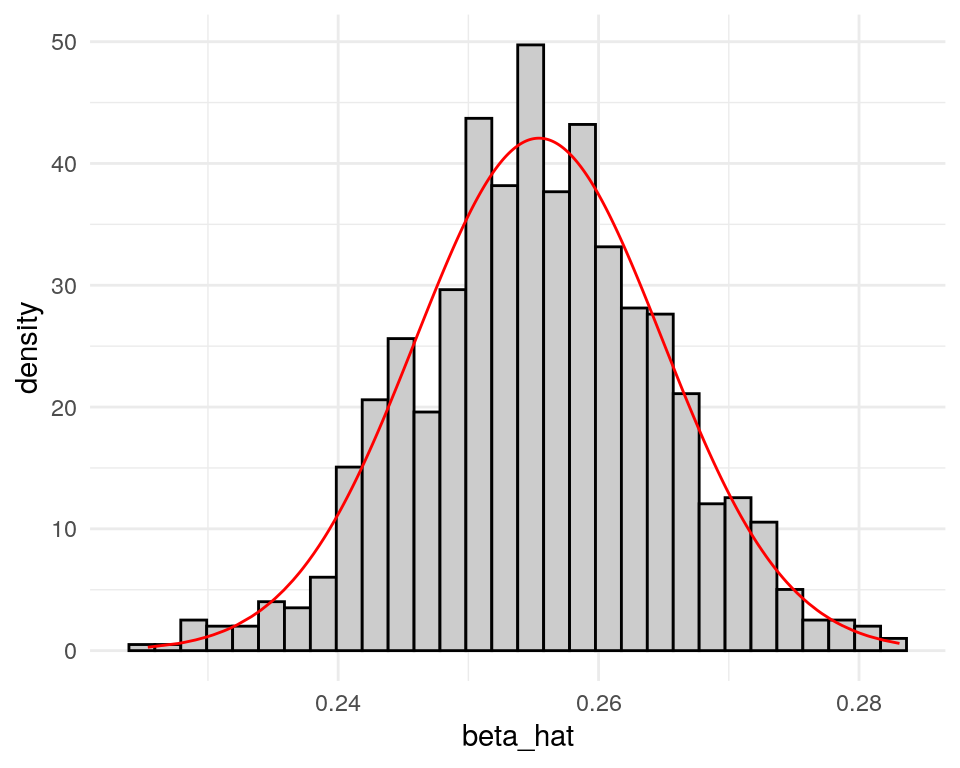
\includegraphics[width=0.7\linewidth]{12Final_files/figure-beamer/unnamed-chunk-4-1}

\end{frame}

\begin{frame}

Hierarchical clustering for visualization

\centering

\includegraphics[width=0.7\textwidth,height=\textheight]{../1Intro/heatmap.png}

\end{frame}

\begin{frame}[fragile]

\begin{block}{11. Neural networks}

\(~\)

\begin{itemize}
\item
  Feedforward network architecture: mathematical formula - layers of
  multivariate transformed (\texttt{relu}, \texttt{linear},
  \texttt{sigmoid}) inner products - sequentially connected.
  \vspace{2mm}
\item
  Loss function to minimize (on output layer): regression (mean
  squared), classification binary (binary crossentropy), classification
  multiple classes (categorical crossentropy). \vspace{2mm}
\item
  Remember the correct choice of output activiation function: mean
  squared loss goes with linear activation, binary crossentropy with
  sigmoid, categorical crossentropy with softmax. \vspace{2mm}
\item
  Gradient based (chain rule) back-propagation - many variants.
  \vspace{2mm}
\item
  The phenomenon of \emph{double descent}. \vspace{2mm}
\item
  \texttt{keras} in R. Use of tensors: Piping sequential layers, piping
  to estimation and then to evaluation (metrics).
\end{itemize}

\end{block}

\end{frame}

\begin{frame}{Mentimeter poll}
\protect\hypertarget{mentimeter-poll}{}

\(~\)

\centering

www.menti.com

Code 3677 2208

\end{frame}

\begin{frame}{Some cautionary words}
\protect\hypertarget{some-cautionary-words}{}

\(~\)

\begin{itemize}
\item
  In most of the problems we looked at we could (or had to) choose a set
  of variables to explain or predict an outcome (\(y\)).
\item
  Model selection was the topic of Module 6, but there is more to say
  about it, in particular in the regression context.
\item
  Importantly, the approach to find a model \textbf{heavily depends on
  the aim} for which the model is built.
\end{itemize}

\(~\)

It is important to make the following distinction:

\begin{itemize}
\tightlist
\item
  The aim is to \emph{\textcolor{red}{predict}} future values of \(y\)
  from known regressors.
\item
  The aim is to \emph{\textcolor{red}{explain}} \(y\) using known
  regressors. In this case, the ultimate aim is to find \emph{causal
  relationships}.
\end{itemize}

\end{frame}

\begin{frame}

\(\rightarrow\) Even among statisticians there is no real consensus
about how, if, or when to select a model:

\vspace{2mm}


\includegraphics[width=0.9\textwidth,height=\textheight]{graphics/brewer_title.png}
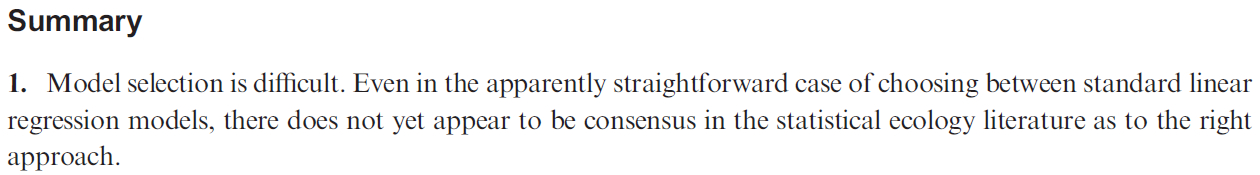
\includegraphics[width=0.9\textwidth,height=\textheight]{graphics/brewer.png}

Note: The first sentence of a paper in \emph{Methods in Ecology and
Evolution} from 2016 is: ``Model selection is difficult.''

\end{frame}

\begin{frame}

\begin{block}{Why is finding a model so hard?}

\(~\)

A model is an approximation of the reality. The aim of statistics and
data analysis is to find connections (explanations or predictions)
thanks to simplifications of the real world.

\(~\)

Box (1979):
\emph{\textcolor{red}{``All models are wrong, but some are useful.''}}

\(~\) \(~\)

\(\rightarrow\) There is often not a ``right'' or a ``wrong'' model --
but there are more and less useful ones.

\(~\)

\(\rightarrow\) Finding a model or the appropriate method with good
properties is sometimes an art\ldots{}

\end{block}

\end{frame}

\begin{frame}

\begin{block}{Predictive and explanatory models}

\(~\)

When choosing a method or a model, you need to be clear about the scope:

\(~\)

\begin{itemize}
\tightlist
\item
  \textbf{\textcolor{red}{Predictive models}}: These are models that aim
  to predict the outcome of future subjects. \vspace{2mm}\\
  \textbf{Example:} In the bodyfat example (module 3) the aim is to
  predict people's bodyfat from factors that are easy to measure (age,
  BMI, weight,..).
\end{itemize}

\(~\)

\begin{itemize}
\tightlist
\item
  \textbf{\textcolor{red}{Explanatory models}}: These are models that
  aim at understanding the (causal) relationship between covariates and
  the response. \vspace{2mm}\\
  \textbf{Example:} The South African heart disease data (module 4) aims
  to identify important risk factors for coronary heart disease.
\end{itemize}

\(~\)

\(\rightarrow\) \textbf{The model selection strategy depends on this
distinction.}

\end{block}

\end{frame}

\begin{frame}

\begin{block}{Prediction vs explanation}

\(~\)

When the aim is \textbf{\emph{prediction}}, the best model is the one
that best predicts the fate of a future subject (smallest test error
rate). This is a well defined task and ``objective'' variable selection
strategies to find the model which is best in this sense are potentially
useful.

\(~\)

However, when used for \textbf{\emph{explanation}} the best model will
depend on the scientific question being asked, \textbf{and automatic
variable selection strategies have no place}.

\(~\)

\scriptsize

Chapters 27.1 and 27.2 in Clayton and Hills (1993)

\end{block}

\end{frame}

\begin{frame}

\begin{block}{Model selection with AIC, AIC\(_c\), BIC, \(C_p\),
adjusted \(R^2\)}

\(~\)

Given \(m\) potential variables to be included in a model. Remember from
Module 6: \vspace{2mm}

\begin{itemize}
\item
  Subset selection using forward, backward or best subset selection
  method.
\item
  Use an ``objective'' criterion to find the ``best'' model.
\end{itemize}

\(~\)

\textbf{Cautionary Note}:

The coefficients of such an optimized ``best'' model should \emph{not be
interpreted} in a causal sense! Why?

\(~\)

\begin{itemize}
\tightlist
\item
  Subset selection may lead to \textbf{biased parameter estimates}, thus
  \textbf{do not draw (biological, medical,..) conclusions} from models
  that were optimized for prediction, for example by AIC/AICc/BIC
  minimization! See, e.g., Freedman (1983), Copas (1983).
\end{itemize}

\vspace{2mm}
\normalsize

\end{block}

\end{frame}

\begin{frame}[fragile]

\begin{block}{Illustration: Model selection bias}

\(~\)

\textbf{Aim of the example:} To illustrate how model selection purely
based on AIC can lead to biased parameters and overestimated effects.

\(~\)

\emph{Procedure:} \vspace{2mm}

\begin{enumerate}
\tightlist
\item
  Randomly generate 100 data points for 50 covariables
  \(x^{(1)},\ldots, x^{(50)}\) and a response \(y\):
\end{enumerate}

\(~\) \scriptsize

\begin{Shaded}
\begin{Highlighting}[]
\KeywordTok{set.seed}\NormalTok{(}\DecValTok{123456}\NormalTok{)}
\NormalTok{data_aic <-}\StringTok{ }\KeywordTok{data.frame}\NormalTok{(}\KeywordTok{matrix}\NormalTok{(}\KeywordTok{rnorm}\NormalTok{(}\DecValTok{51} \OperatorTok{*}\StringTok{ }\DecValTok{100}\NormalTok{), }\DataTypeTok{ncol =} \DecValTok{51}\NormalTok{))}
\KeywordTok{names}\NormalTok{(data_aic)[}\DecValTok{51}\NormalTok{] <-}\StringTok{ "Y"}
\end{Highlighting}
\end{Shaded}

\(~\)

\normalsize

\texttt{data} is a 100\(\times\) 51 matrix, where the last column is the
response. The \textbf{data were generated completely independently}, the
covariates do not have any explanatory power for the response!

\end{block}

\end{frame}

\begin{frame}[fragile]

\begin{enumerate}
\setcounter{enumi}{1}
\tightlist
\item
  Fit a linear regression model of \(y\) against all the 50 variables
  \begin{equation*}
  y_i = \beta_0 + \beta_1 x_i^{(1)} + \ldots + \beta_{50}x_i^{(50)} + \epsilon_i \ .
  \end{equation*}
\end{enumerate}

\scriptsize

\begin{Shaded}
\begin{Highlighting}[]
\NormalTok{r.lm.aic <-}\StringTok{ }\KeywordTok{lm}\NormalTok{(Y }\OperatorTok{~}\StringTok{ }\NormalTok{., data_aic)}
\end{Highlighting}
\end{Shaded}

\normalsize

As expected, the distribution of the \(p\)-values is (more or less)
uniform between 0 and 1, with none below 0.05:

\scriptsize
\center

\begin{Shaded}
\begin{Highlighting}[]
\KeywordTok{hist}\NormalTok{(}\KeywordTok{summary}\NormalTok{(r.lm.aic)}\OperatorTok{$}\NormalTok{coef[}\OperatorTok{-}\DecValTok{1}\NormalTok{, }\DecValTok{4}\NormalTok{], }\DataTypeTok{freq =}\NormalTok{ T, }\DataTypeTok{main =} \StringTok{"50 variables"}\NormalTok{, }
    \DataTypeTok{xlab =} \StringTok{"p-values"}\NormalTok{)}
\end{Highlighting}
\end{Shaded}

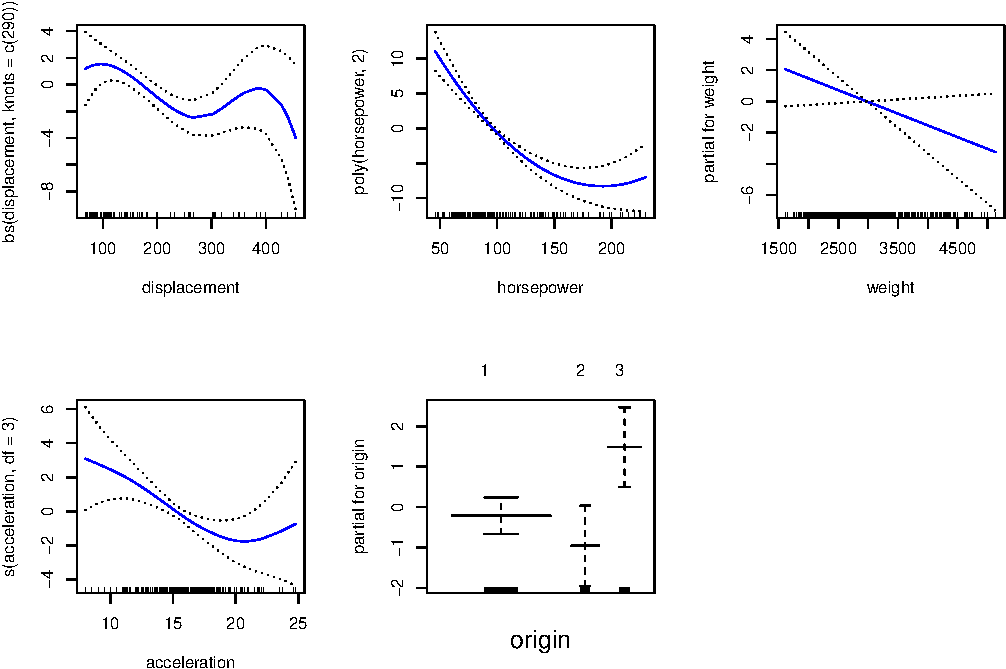
\includegraphics[width=4cm]{12Final_files/figure-beamer/unnamed-chunk-7-1}

\end{frame}

\begin{frame}[fragile]

\begin{enumerate}
\setcounter{enumi}{2}
\tightlist
\item
  Then use AICc minimization to obtain the objectively ``best'' model:
\end{enumerate}

\vspace{2mm}

\scriptsize

\begin{Shaded}
\begin{Highlighting}[]
\KeywordTok{library}\NormalTok{(MASS)}
\NormalTok{r.AICmin <-}\StringTok{ }\KeywordTok{stepAIC}\NormalTok{(r.lm.aic, }\DataTypeTok{direction =} \KeywordTok{c}\NormalTok{(}\StringTok{"both"}\NormalTok{), }\DataTypeTok{trace =} \OtherTok{FALSE}\NormalTok{, }\DataTypeTok{AICc =} \OtherTok{TRUE}\NormalTok{)}
\end{Highlighting}
\end{Shaded}

\centering

\begin{Shaded}
\begin{Highlighting}[]
\KeywordTok{hist}\NormalTok{(}\KeywordTok{summary}\NormalTok{(r.AICmin)}\OperatorTok{$}\NormalTok{coef[}\OperatorTok{-}\DecValTok{1}\NormalTok{, }\DecValTok{4}\NormalTok{], }\DataTypeTok{freq =}\NormalTok{ T, }\DataTypeTok{main =} \StringTok{"18 variables of minimal AICc model"}\NormalTok{, }
    \DataTypeTok{xlab =} \StringTok{"p-values"}\NormalTok{)}
\end{Highlighting}
\end{Shaded}

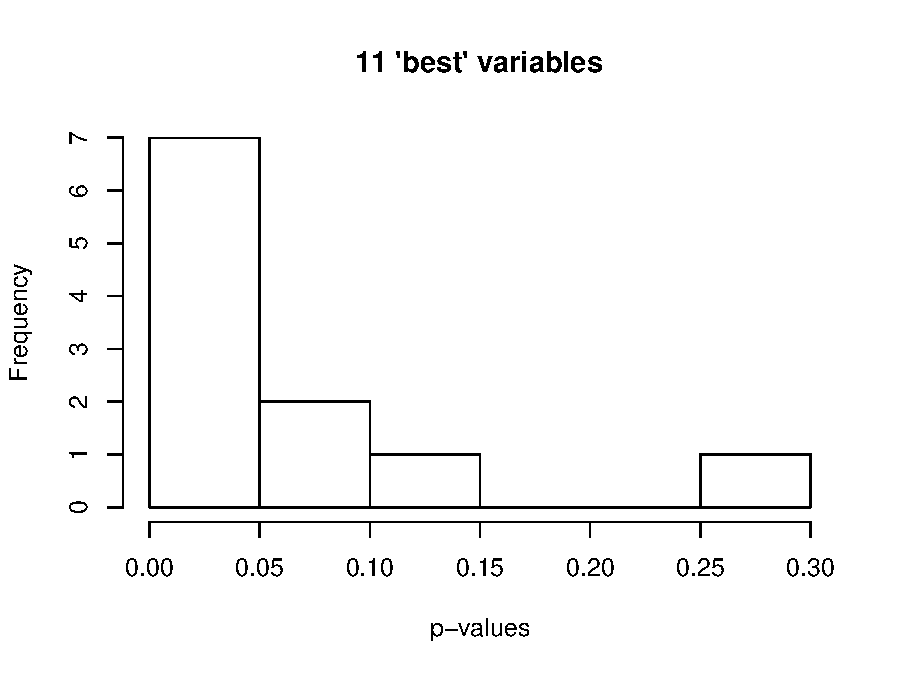
\includegraphics[width=4cm]{12Final_files/figure-beamer/unnamed-chunk-9-1}

\flushleft
\normalsize

The distribution of the \(p\)-values is now skewed: many of them reach
rather small values (7 have \(p<0.05\)). This happened \emph{although
none of the variables has any explanatory power!}

\end{frame}

\begin{frame}

\begin{block}{Summary: Main problem with model selection}

\(~\)

\colorbox{lightgray}{\begin{minipage}{10cm}
When model selection is carried out based on objective criteria, the effect sizes will to be too large and the uncertainty too small. So you end up being too sure about a too large effect. 
\end{minipage}}

\(~\)

\(~\)

\textbf{Exception}: Shrinkage methods!

\end{block}

\end{frame}

\begin{frame}

Which methods are suitable for explanation (inference)? \vspace{-2mm}

\centering

\includegraphics{../../ISLR/Figures/Chapter2/2.7.png}

\end{frame}

\begin{frame}

\begin{block}{Bottomline}

\(~\)

\begin{itemize}
\tightlist
\item
  \emph{Less flexible} models tend to have \emph{better
  interpretability} and are therefore better suited \emph{for
  explanation} than more flexible models.
\end{itemize}

\vspace{2mm}

\begin{itemize}
\tightlist
\item
  The \emph{more flexible} a model, the better it tends to perform
  \emph{for prediction}.
\end{itemize}

\vspace{2mm}

\begin{itemize}
\tightlist
\item
  Some models can be used for both, prediction and explanation, but then
  the approach how to build the model (e.g., how to select variables)
  should still depend on the aim.
\end{itemize}

Thank you for attending this course - good luck for the exam!

\end{block}

\end{frame}

\begin{frame}{References}
\protect\hypertarget{references}{}

\hypertarget{refs}{}
\leavevmode\hypertarget{ref-clayton.hills1993}{}%
Clayton, D., and M. Hills. 1993. \emph{Statistical Models in
Epidemiology}. Oxford: Oxford University Press.

\leavevmode\hypertarget{ref-copas1983}{}%
Copas, J. B. 1983. ``Regression, Prediction and Shrinkage.''
\emph{Journal of the Royal Statistical Society. Series B (Statistical
Methodology)} 45: 311--54.

\leavevmode\hypertarget{ref-freedman1983}{}%
Freedman, D. A. 1983. ``A Note on Screening Regression Equations.''
\emph{The American Statistician} 37: 152--55.

\leavevmode\hypertarget{ref-ISL}{}%
James, Gareth, Daniela Witten, Trevor Hastie, and Robert Tibshirani.
2013. \emph{An Introduction to Statistical Learning}. Vol. 112.
Springer.

\leavevmode\hypertarget{ref-james.etal}{}%
James, G., D. Witten, T. Hastie, and R. Tibshirani. 2013. \emph{An
Introduction to Statistical Learning with Applications in R}. New York:
Springer.

\end{frame}

\end{document}
